\section{Channel System}
\label{sec:channelSystem}

To justify and motivate the use of a CS, we need to establish our requirements. Recalling our motivation example (Section \ref{sec:motivation}), the team's members execute tasks in parallel and each member exchange information with the leader, changing its decisions based on the instructions its receives, i.e, which tasks are allocated for it. Moreover, dynamic events also changes its attitudes, e.g, sensor failure causes an information exchange with the leader, to update the task allocation process. Thus, the capability of coping with context changes eventually arising during a mission in a \textit{nondeterministic} way motivate the use of \textit{program graphs}~\cite{modelcheckingBaier}. Furthermore, the execution of parallel processes and the communication among members are requirements that prompt the use of \textit{channel systems}~\cite{modelcheckingBaier}.

A channel system is composed of a group of data-dependent processes communicating with each other via \textit{communication actions}~\cite{modelcheckingBaier}. With a program graph representing each process, transitions among states can be classified between conditional transitions or communication actions. Conditional transitions are important to avoid transitioning to states undesirably, according to boolean evaluations~\cite{modelcheckingBaier} defined during planning. The last type of transition works transmitting values through channels or receiving values from channels and assigning them to variables~\cite{modelcheckingBaier}. Additionally, channels can have a finite or infinite capacity of messages in a single channel, as well as a specified type of messages that can be stored in it. Finally, channel systems provide a notion of synchronization, whereas channels with a capacity different from zero function in a \textit{asynchronous} way and null capacity channels represent \textit{synchronous} communication~\cite{modelcheckingBaier}.

\begin{figure}[!ht]
    \centering
    \scalebox{.75}{\section{Channel System}
\label{sec:channelSystem}}
    \caption{Proposed Channel System}
    \label{fig:CS}
\end{figure}

Figure \ref{fig:CS} illustrates our channel system. The proposed channel system describes our coordination strategy. We decided to model our coordination using separate roles, mainly due to its nature of modulatizing functional aspects~\cite{roleOrientedModeling}. Also, roles are used to define positions within an organization, encapsulating certain tasks, responsibilities, and goals that an owner of a role has to fulfil~\cite{roleOrientedModeling}. Thus, each member of the team can posses a program graph that describes a distinct role, and more than one role can coexist in the same entity. Also, during maneuvering between different C2 approaches~\cite{france2014}, roles assignment can be changed, providing more possibilities to the team during the mission.

To modularize roles, we divided the coordination aspect among two different roles:

\begin{itemize}
    \item Task Allocator (TA): responsible for distributing tasks throughout the team, based on team members attributes, such as fuel and sensors onboard. Moreover, this role reports results provided by executors to the C2 approach selector role;
    \item C2 Approach Selector (C2S): responsible for detecting the need of changing the C2 approach, due to some drop in performance reported by task allocator. Additionally, it communicates to task allocator if a maneuver will occur.  
\end{itemize}

Furthermore, each member executes its set of roles encapsulated in it. For instance, as depicted in Figure \ref{fig:CS}, each member playing the executor (EX) role communicates with the leader, i.e, member who plays the role TA, using channel \textit{$ch_1$} in a asynchronous manner. Similarly, the leader provides tasks to each executor member using channel \textit{$m_i$} whereas $i$ is the executor's index. Finally, the C2S role and TA role exchange information using synchronized channels \textit{$ch_2$} and \textit{$ch_3$} to asses performance and check if a maneuver is crucial to maintain quality of execution during the mission. These latter channels use synchronized communication because the TA role provides performance information using channel \textit{$ch_3$} and waits for the C2S's response to know if a maneuver might happen. Until this feedback information approaches the channel \textit{$ch_2$}, the TA role stops allocating tasks to the remaining members. However, members that execute tasks, i.e, play the EX role, and allocate tasks, i.e, play the TA role, don't need to wait for any response and can continue executing tasks or allocating tasks, justifying the asynchronous communication between these roles.

\begin{figure}[!ht]
    \centering
    \scalebox{.65}{

\tikzset{every picture/.style={line width=0.75pt}} %set default line width to 0.75pt        

\begin{tikzpicture}[x=0.75pt,y=0.75pt,yscale=-1,xscale=1]
%uncomment if require: \path (0,754); %set diagram left start at 0, and has height of 754

%Curve Lines [id:da9480858267519683] 
\draw    (230.5,181) .. controls (264.16,138.43) and (373.78,135.06) .. (406.05,178.66) ;
\draw [shift={(407,180)}, rotate = 235.44] [color={rgb, 255:red, 0; green, 0; blue, 0 }  ][line width=0.75]    (10.93,-3.29) .. controls (6.95,-1.4) and (3.31,-0.3) .. (0,0) .. controls (3.31,0.3) and (6.95,1.4) .. (10.93,3.29)   ;
%Shape: Ellipse [id:dp6594609066072359] 
\draw   (120.5,208) .. controls (120.5,194.19) and (147.14,183) .. (180,183) .. controls (212.86,183) and (239.5,194.19) .. (239.5,208) .. controls (239.5,221.81) and (212.86,233) .. (180,233) .. controls (147.14,233) and (120.5,221.81) .. (120.5,208) -- cycle ;
%Shape: Ellipse [id:dp873836537729809] 
\draw   (397,201.5) .. controls (397,187.42) and (423.53,176) .. (456.25,176) .. controls (488.97,176) and (515.5,187.42) .. (515.5,201.5) .. controls (515.5,215.58) and (488.97,227) .. (456.25,227) .. controls (423.53,227) and (397,215.58) .. (397,201.5) -- cycle ;
%Curve Lines [id:da14662580418826565] 
\draw    (514.5,424) .. controls (567.96,419.05) and (594.96,385.68) .. (603.25,341.35) ;
\draw [shift={(603.5,340)}, rotate = 460.08] [color={rgb, 255:red, 0; green, 0; blue, 0 }  ][line width=0.75]    (10.93,-3.29) .. controls (6.95,-1.4) and (3.31,-0.3) .. (0,0) .. controls (3.31,0.3) and (6.95,1.4) .. (10.93,3.29)   ;
%Straight Lines [id:da37650774099478246] 
\draw    (232.5,14) -- (263.11,24.36) ;
\draw [shift={(265,25)}, rotate = 198.7] [color={rgb, 255:red, 0; green, 0; blue, 0 }  ][line width=0.75]    (10.93,-3.29) .. controls (6.95,-1.4) and (3.31,-0.3) .. (0,0) .. controls (3.31,0.3) and (6.95,1.4) .. (10.93,3.29)   ;
%Shape: Ellipse [id:dp8139093405894636] 
\draw   (121,419) .. controls (121,405.19) and (147.53,394) .. (180.25,394) .. controls (212.97,394) and (239.5,405.19) .. (239.5,419) .. controls (239.5,432.81) and (212.97,444) .. (180.25,444) .. controls (147.53,444) and (121,432.81) .. (121,419) -- cycle ;
%Shape: Ellipse [id:dp08678607998247811] 
\draw   (391,418) .. controls (391,404.19) and (417.53,393) .. (450.25,393) .. controls (482.97,393) and (509.5,404.19) .. (509.5,418) .. controls (509.5,431.81) and (482.97,443) .. (450.25,443) .. controls (417.53,443) and (391,431.81) .. (391,418) -- cycle ;
%Shape: Ellipse [id:dp07482494496489733] 
\draw   (270,28) .. controls (270,14.75) and (296.53,4) .. (329.25,4) .. controls (361.97,4) and (388.5,14.75) .. (388.5,28) .. controls (388.5,41.25) and (361.97,52) .. (329.25,52) .. controls (296.53,52) and (270,41.25) .. (270,28) -- cycle ;
%Curve Lines [id:da6759956440889884] 
\draw    (123.5,226) .. controls (100.84,271.31) and (108.27,364.16) .. (126.65,401.34) ;
\draw [shift={(127.5,403)}, rotate = 242.18] [color={rgb, 255:red, 0; green, 0; blue, 0 }  ][line width=0.75]    (10.93,-3.29) .. controls (6.95,-1.4) and (3.31,-0.3) .. (0,0) .. controls (3.31,0.3) and (6.95,1.4) .. (10.93,3.29)   ;
%Curve Lines [id:da9572857730465772] 
\draw    (234.22,228.76) .. controls (260.54,268.31) and (261.61,376.42) .. (236,404) ;
\draw [shift={(233,227)}, rotate = 54.11] [color={rgb, 255:red, 0; green, 0; blue, 0 }  ][line width=0.75]    (10.93,-3.29) .. controls (6.95,-1.4) and (3.31,-0.3) .. (0,0) .. controls (3.31,0.3) and (6.95,1.4) .. (10.93,3.29)   ;
%Curve Lines [id:da9385545433271328] 
\draw    (517.5,315) .. controls (479.88,326.88) and (463.82,339.74) .. (457.68,385.6) ;
\draw [shift={(457.5,387)}, rotate = 277.28] [color={rgb, 255:red, 0; green, 0; blue, 0 }  ][line width=0.75]    (10.93,-3.29) .. controls (6.95,-1.4) and (3.31,-0.3) .. (0,0) .. controls (3.31,0.3) and (6.95,1.4) .. (10.93,3.29)   ;
%Curve Lines [id:da13526468384837043] 
\draw    (440.5,173) .. controls (426.78,119.1) and (401.54,70) .. (377.94,50.18) ;
\draw [shift={(376.5,49)}, rotate = 398.37] [color={rgb, 255:red, 0; green, 0; blue, 0 }  ][line width=0.75]    (10.93,-3.29) .. controls (6.95,-1.4) and (3.31,-0.3) .. (0,0) .. controls (3.31,0.3) and (6.95,1.4) .. (10.93,3.29)   ;
%Curve Lines [id:da7876400787103589] 
\draw    (267.5,45) .. controls (238.79,63.81) and (213.02,106.14) .. (201.83,170.06) ;
\draw [shift={(201.5,172)}, rotate = 279.61] [color={rgb, 255:red, 0; green, 0; blue, 0 }  ][line width=0.75]    (10.93,-3.29) .. controls (6.95,-1.4) and (3.31,-0.3) .. (0,0) .. controls (3.31,0.3) and (6.95,1.4) .. (10.93,3.29)   ;
%Shape: Ellipse [id:dp538933115831977] 
\draw   (524,310) .. controls (524,296.19) and (550.3,285) .. (582.75,285) .. controls (615.2,285) and (641.5,296.19) .. (641.5,310) .. controls (641.5,323.81) and (615.2,335) .. (582.75,335) .. controls (550.3,335) and (524,323.81) .. (524,310) -- cycle ;
%Curve Lines [id:da663291454681702] 
\draw    (518.5,205) .. controls (566.52,205) and (582.85,245.34) .. (584.42,278.01) ;
\draw [shift={(584.5,280)}, rotate = 268.26] [color={rgb, 255:red, 0; green, 0; blue, 0 }  ][line width=0.75]    (10.93,-3.29) .. controls (6.95,-1.4) and (3.31,-0.3) .. (0,0) .. controls (3.31,0.3) and (6.95,1.4) .. (10.93,3.29)   ;
%Curve Lines [id:da17641910717404863] 
\draw    (413.5,391) .. controls (394.69,323.68) and (299.43,241.66) .. (246.1,216.74) ;
\draw [shift={(244.5,216)}, rotate = 384.36] [color={rgb, 255:red, 0; green, 0; blue, 0 }  ][line width=0.75]    (10.93,-3.29) .. controls (6.95,-1.4) and (3.31,-0.3) .. (0,0) .. controls (3.31,0.3) and (6.95,1.4) .. (10.93,3.29)   ;
%Rounded Rect [id:dp2887172897272543] 
\draw   (49,521.88) .. controls (49,514.76) and (54.76,509) .. (61.88,509) -- (626.12,509) .. controls (633.24,509) and (639,514.76) .. (639,521.88) -- (639,729.12) .. controls (639,736.24) and (633.24,742) .. (626.12,742) -- (61.88,742) .. controls (54.76,742) and (49,736.24) .. (49,729.12) -- cycle ;
%Rounded Rect [id:dp07131134126212679] 
\draw   (13.5,469.8) .. controls (13.5,465.49) and (16.99,462) .. (21.3,462) -- (658.7,462) .. controls (663.01,462) and (666.5,465.49) .. (666.5,469.8) -- (666.5,493.2) .. controls (666.5,497.51) and (663.01,501) .. (658.7,501) -- (21.3,501) .. controls (16.99,501) and (13.5,497.51) .. (13.5,493.2) -- cycle ;
%Curve Lines [id:da580151899278355] 
\draw    (128,189) .. controls (100.91,166.34) and (132.04,140.78) .. (153.05,178.24) ;
\draw [shift={(154,180)}, rotate = 242.3] [color={rgb, 255:red, 0; green, 0; blue, 0 }  ][line width=0.75]    (10.93,-3.29) .. controls (6.95,-1.4) and (3.31,-0.3) .. (0,0) .. controls (3.31,0.3) and (6.95,1.4) .. (10.93,3.29)   ;

% Text Node
\draw (181,207) node   [align=left] {Ready};
% Text Node
\draw (457,200) node   [align=left] {Allocating};
% Text Node
\draw (323,167) node    {$T'\ \neq [] :allocate$};
% Text Node
\draw (182,419) node   [align=left] {Updating};
% Text Node
\draw (584,308) node   [align=left] {Notifying};
% Text Node
\draw (330,29) node   [align=left] {Waiting};
% Text Node
\draw (71,319) node    {$ch_{1} ?\langle t,e' \rangle $};
% Text Node
\draw (221,303) node    {$update$};
% Text Node
\draw (487,84) node    {$alloc=[] :ch_{3} !\langle T',E'\rangle $};
% Text Node
\draw (188,79) node    {$ch_{2} ?\langle T',E'\rangle $};
% Text Node
\draw (452,418) node   [align=left] {Binding};
% Text Node
\draw (599,426) node    {$alloc\neq [] :bind$};
% Text Node
\draw (445,327) node    {$m_{k\ } !\ T'_{k}$};
% Text Node
\draw (596,195) node    {$alloc\neq [] :bind$};
% Text Node
\draw (391,266) node    {$alloc=[] :done$};
% Text Node
\draw (346,622) node    {$ \begin{array}{l}
Var=\{\ alloc:[ \langle \ \mathbb{N} ,[ Task] \ \rangle ] ;\ f\_alloc:([ Task] ,[ FM] ,C2_{ap}) \ \rightarrow [ \langle \ \mathbb{N} ,[ Task] \ \rangle ] ;\ \\
\ \ \ \ \ \ \ \ \ \ \ \ teamStatus:[ FM] \ \rightarrow \ \langle [ Task] ,[ FM] \rangle ;\ T':[ Task] ;\ T_{success} :[ Task] ;\ \\
\ \ \ \ \ \ \ \ \ \ \ \ E':[ FM] ;\ t:Task;\ e' :FM;\ \omega :C2_{ap} ;\ T_{add} :[ Task] \ \}\\
Effect( allocate,\ \eta ) =\ \eta [ alloc:=\ f\_alloc( T',\ E',\ \omega )]\\
Effect( bind,\ \eta ) =\ \eta [ \ \langle k,T'_{k} \rangle :=head( alloc) ;\ alloc:=tail( alloc) \ ]\\
Effect( update,\ \eta ) =\begin{cases}
\eta [ \ T_{success} :=T_{success} \ ++\ [ t] \ ] & \ \ \ \ if\ ( e'=null)\\
\eta [ \ T':=T'++\ [ t] \ ;\ E':=E'( e/e'_{\ })] & \ \ \ \ otherwise
\end{cases} \ \\
Effect( done,\eta ) =\eta [ \ T':=[] \ ]\\
Effect( memberFailure,\eta ) =\eta [ \ \langle T',E'\rangle :=teamStatus( E') \ ]
\end{array}$};
% Text Node
\draw (219,8) node    {$g_{0}$};
% Text Node
\draw (342.76,480) node    {$g_{0} :=( T'=[]) \ \land ( f\_alloc\ =\ f_{x}([ t_{1} ,\ ...,t_{n}] \ p_{1} ,\ [ e_{1} ,...,e_{n}] \ p_{2})) \ \land ( T_{success} =[]) \ \land \ ( \omega =\omega _{0})$};
% Text Node
\draw (97,144) node    {$memberFailure$};


\end{tikzpicture}}
    \caption{Task Allocator Role Program Graph}
    \label{fig:TA}
\end{figure}

Figure \ref{fig:TA} illustrates the TA role's program graph. It receives a set of variables, e.g, $T'$ and $E'$, from the C2S role, transitioning from location "Waiting" to "Ready". Some actions to switch between locations are conditional, e.g, to advance from location "Ready" to location "Allocating" the action $allocate$ can be executed, depending on the comparison between the set of available tasks, $T'$, and an empty set. So, if there are still tasks available, it execute $allocate$ and proceed to location "Allocating". The action $allocate$ results in assigning to variable $alloc$ the return of the function $f\_alloc$. This last function is specified at line 1 of our variables and functions definitions description. In summary, $alloc$ is assigned a list of pairs, each with an index of a team member and a list of tasks designated to it. To build this list, $f\_alloc$ uses the set of available tasks, $T'$, the set of team members attributes, $E'$, and the current C2 approach, $\omega$, as inputs to perform the task assignment using some criteria established during planning.

\begin{figure}[!ht]
    \centering
    \scalebox{.65}{

\tikzset{every picture/.style={line width=0.75pt}} %set default line width to 0.75pt        

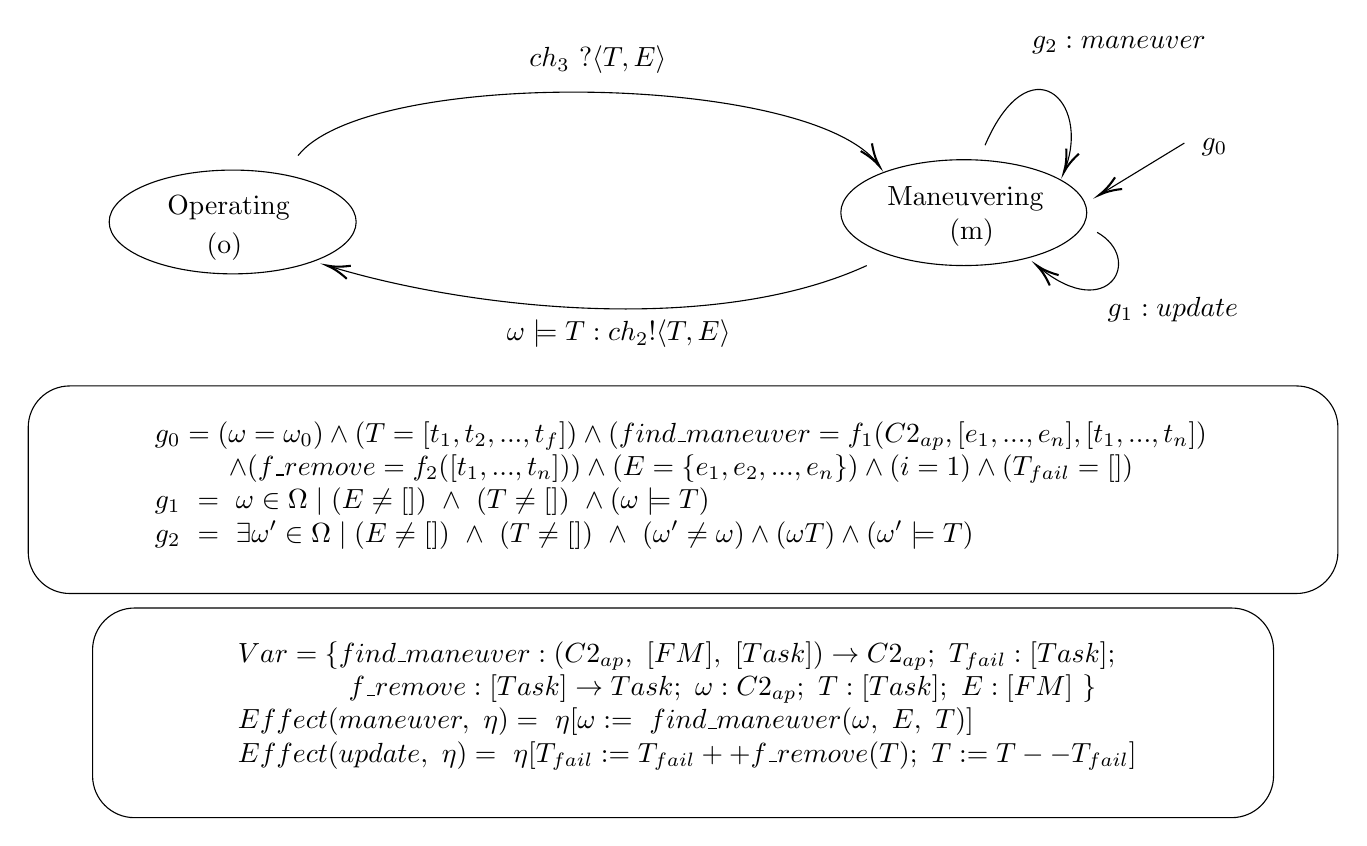
\begin{tikzpicture}[x=0.75pt,y=0.75pt,yscale=-1,xscale=1]
%uncomment if require: \path (0,397); %set diagram left start at 0, and has height of 397

%Curve Lines [id:da9480858267519683] 
\draw    (135.5,66) .. controls (169.16,23.43) and (380.22,25.94) .. (414.52,69.66) ;
\draw [shift={(415.5,71)}, rotate = 235.44] [color={rgb, 255:red, 0; green, 0; blue, 0 }  ][line width=0.75]    (10.93,-3.29) .. controls (6.95,-1.4) and (3.31,-0.3) .. (0,0) .. controls (3.31,0.3) and (6.95,1.4) .. (10.93,3.29)   ;
%Shape: Ellipse [id:dp6594609066072359] 
\draw   (44.5,98) .. controls (44.5,84.19) and (71.14,73) .. (104,73) .. controls (136.86,73) and (163.5,84.19) .. (163.5,98) .. controls (163.5,111.81) and (136.86,123) .. (104,123) .. controls (71.14,123) and (44.5,111.81) .. (44.5,98) -- cycle ;
%Shape: Ellipse [id:dp873836537729809] 
\draw   (397,93.5) .. controls (397,79.42) and (423.53,68) .. (456.25,68) .. controls (488.97,68) and (515.5,79.42) .. (515.5,93.5) .. controls (515.5,107.58) and (488.97,119) .. (456.25,119) .. controls (423.53,119) and (397,107.58) .. (397,93.5) -- cycle ;
%Curve Lines [id:da21020703050779688] 
\draw    (466.5,61) .. controls (487.68,11.75) and (517.59,39.15) .. (505.1,72.47) ;
\draw [shift={(504.5,74)}, rotate = 292.38] [color={rgb, 255:red, 0; green, 0; blue, 0 }  ][line width=0.75]    (10.93,-3.29) .. controls (6.95,-1.4) and (3.31,-0.3) .. (0,0) .. controls (3.31,0.3) and (6.95,1.4) .. (10.93,3.29)   ;
%Curve Lines [id:da14662580418826565] 
\draw    (520.5,103) .. controls (543.16,115.81) and (526.03,147.04) .. (493.02,120.26) ;
\draw [shift={(491.5,119)}, rotate = 400.46000000000004] [color={rgb, 255:red, 0; green, 0; blue, 0 }  ][line width=0.75]    (10.93,-3.29) .. controls (6.95,-1.4) and (3.31,-0.3) .. (0,0) .. controls (3.31,0.3) and (6.95,1.4) .. (10.93,3.29)   ;
%Straight Lines [id:da37650774099478246] 
\draw    (562.5,60) -- (523.21,83.96) ;
\draw [shift={(521.5,85)}, rotate = 328.63] [color={rgb, 255:red, 0; green, 0; blue, 0 }  ][line width=0.75]    (10.93,-3.29) .. controls (6.95,-1.4) and (3.31,-0.3) .. (0,0) .. controls (3.31,0.3) and (6.95,1.4) .. (10.93,3.29)   ;
%Rounded Rect [id:dp20897962983691354] 
\draw   (5.5,197) .. controls (5.5,185.95) and (14.45,177) .. (25.5,177) -- (616.5,177) .. controls (627.55,177) and (636.5,185.95) .. (636.5,197) -- (636.5,257) .. controls (636.5,268.05) and (627.55,277) .. (616.5,277) -- (25.5,277) .. controls (14.45,277) and (5.5,268.05) .. (5.5,257) -- cycle ;
%Rounded Rect [id:dp6489541210438411] 
\draw   (36.5,304.2) .. controls (36.5,293.04) and (45.54,284) .. (56.7,284) -- (585.3,284) .. controls (596.46,284) and (605.5,293.04) .. (605.5,304.2) -- (605.5,364.8) .. controls (605.5,375.96) and (596.46,385) .. (585.3,385) -- (56.7,385) .. controls (45.54,385) and (36.5,375.96) .. (36.5,364.8) -- cycle ;
%Curve Lines [id:da13961356622291943] 
\draw    (409.5,119) .. controls (335.87,152.83) and (218.68,140.13) .. (150.52,119.31) ;
\draw [shift={(149.5,119)}, rotate = 377.15999999999997] [color={rgb, 255:red, 0; green, 0; blue, 0 }  ][line width=0.75]    (10.93,-3.29) .. controls (6.95,-1.4) and (3.31,-0.3) .. (0,0) .. controls (3.31,0.3) and (6.95,1.4) .. (10.93,3.29)   ;

% Text Node
\draw (102,91) node   [align=left] {Operating};
% Text Node
\draw (457,87) node   [align=left] {Maneuvering};
% Text Node
\draw (280,20) node    {$ch_{3} \ ?\langle T,E\rangle $};
% Text Node
\draw (577,62) node    {$g_{0}$};
% Text Node
\draw (557,140) node    {$g_{1} :update$};
% Text Node
\draw (531,13) node    {$g_{2} :maneuver$};
% Text Node
\draw (320,225) node    {$ \begin{array}{l}
g_{0} =( \omega =\omega _{0}) \land ( T=[ t_{1} ,t_{2} ,...,t_{f}]) \land ( find\_maneuver=f_{1}( C2_{ap} ,[ e_{1} ,...,e_{n}] ,[ t_{1} ,...,t_{n}])\\
\ \ \ \ \ \ \ \ \land ( f\_remove=f_{2}([ t_{1} ,...,t_{n}])) \land ( E=\{e_{1} ,e_{2} ,...,e_{n}\}) \land ( i=1) \land ( T_{fail} =[])\\
g_{1} \ =\ \nexists \omega \in \Omega \mid ( E\neq []) \ \land \ ( T\neq []) \ \land ( \omega \models T) \ \\
g_{2} \ =\ \exists \omega '\in \Omega \mid ( E\neq []) \ \land \ ( T\neq []) \ \land \ ( \omega '\neq \omega ) \land ( \omega \nvDash T) \land ( \omega '\models T)
\end{array}$};
% Text Node
\draw (460,103) node   [align=left] {(m)};
% Text Node
\draw (100,110) node   [align=left] {(o)};
% Text Node
\draw (323,331) node    {$ \begin{array}{l}
Var=\{find\_maneuver:( C2_{ap} ,\ [ FM] ,\ [ Task])\rightarrow C2_{ap} ;\ T_{fail} :[ Task] ;\ \\
\ \ \ \ \ \ \ \ \ \ \ \ f\_remove:[ Task]\rightarrow Task;\ \omega :C2_{ap} ;\ T:[ Task] ;\ E:[ FM] \ \}\\
Effect( maneuver,\ \eta ) =\ \eta [ \omega :=\ find\_maneuver( \omega ,\ E,\ T)]\\
Effect( update,\ \eta ) =\ \eta [ T_{fail} :=T_{fail} ++f\_remove( T) ;\ T:=T--T_{fail}]
\end{array}$};
% Text Node
\draw (290,152) node    {$\omega \models T:ch_{2} !\langle T,E\rangle $};


\end{tikzpicture}}
    \caption{C2 Approach Selector Role Program Graph}
    \label{fig:C2S}
\end{figure}